%\documentclass[10pt, english, pdftex]{template/UC3M_document}
 \documentclass[10pt, spanish, pdftex]{template/UC3M_document}

%%%%%%%%%%%%%%%%%%%%%%%%%%%%%%%%%%%%%%%%%%%%%%%%%%%%%%%%
%               UC3M Work report template              %
%           Universidad Carlos III de Madrid           %
%              Author: Aitor Alonso Núñez              %
%              Last update: January 2019               %
%%%%%%%%%%%%%%%%%%%%%%%%%%%%%%%%%%%%%%%%%%%%%%%%%%%%%%%%

%%%%% Preamble %%%%%
\author{Lucía Ruz}         % This is me! You should write here your name (for PDF metadata)
%%%%% About the authors (will be used on title page and header) %%%%%

%%% Indicate the number of authors by uncommenting the right option.
% \authorstwotrue     % 1 or 2 authors
\authorsthreetrue   % 3 authors
%\authorsfourtrue    % 4 authors

%%% Fill with the authors data. You can leave empty keys {} if you need to and also if you provide more info that number of authors indicated it will be ignored.
% If you selected \authorstwotrue or \authorsthreetrue (1 to 3 authors)
\authorsuptothree{Santiago Ramos Sevillano}{NIA 100383401}{Gr. 83}{Iván Valvuena Gálvez}{NIA 100383375}{Gr. 83}{Lucía Ruz Sáez}{NIA 100363940}{Gr. 83}
% If you selected \coauthorsfourtrue (4 authors)
%\authorsfour{Name1 Lastname1}{NIA 100XXXXXX}{Name2 Lastname2}{NIA 100XXXXXX}{Name3 Lastname3}{NIA 100XXXXXX}{Name4 Lastname4}{NIA 100XXXXXX}{Group XX}

%%% If you want to show coauthors email address on the title page, uncomment \emailtrue. Comment it otherwise.
\emailtrue
% You can leave empty keys {} if you need to and also if you provide more info that number of authors indicated or \emailtrue is commented it will be ignored.
\emails{100383401@alumnos.uc3m.es}{100383375@alumnos.uc3m.es}{100363940@alumnos.uc3m.es}{}


%%%%% Basic data about the document (Degree, subject, title, campus, page number custom text) %%%%%
\documentdata{Ingeniería Informática}{Diseño de Sistemas Operativos}{Practica 1: Planificación de procesos}{EPS}{Page }

%%%%% Page style %%%%%
\header
\footer
\pagestyle{fancy}

\begin{document}
%%%%% Page title %%%%%
\titleMain

%%%%% Index %%%%%
\begin{spacing}{0.5}
    % \shipout\null                   % Blank page before index (after title page)
    \hypersetup{linkcolor=black}    % References/links on the index will remain black color
    \tableofcontents        % Index of the document
    \vspace{1cm}
    \listoffigures\newpage          % Index of pictures
    % \listoftables\newpage           % Index of tables
\end{spacing}


%%%%% DOCUMENT CONTENT %%%%%
\section{Introducción}
A través del presente documento se van a definir los pasos seguidos para el desarrollo de \textbf{tres algoritmos de planificación de hilos en el espacio de usuario}, los cuales se encuentran escritos en el lenguaje de programación C. Estos planificadores han sido creados siguiendo, tanto las pautas dadas en el enunciado de la práctica, como aquellos conocimientos básicos impartidos en la asignatura \textit{Diseño de Sistemas Operativos}.

En primer lugar, es necesario recordar que todos los \textbf{cambios de contexto} en la planificación de procesos de esta práctica se van a realizar en \textbf{espacio de usuario}.

El primer planificador es \textbf{Round-Robin}. El objetivo de esta política es que cada hilo ejecuta un número determinado de rodajas definidas, y una vez terminado dicho número de paso al siguiente hilo listo para ejecutar. El documento final donde se encuentra el código de dicho planificador será nombrado como \textbf{\textit{RR.c}}.

Por otro lado, la segunda política ha de ser \textbf{Round-Robin}, para aquellos hilos con prioridad baja, y \textbf{Shortest Job First con prioridades}, para aquellos hilos de prioridad alta. La política Short Job First ejecuta, en primer lugar, aquellos trabajos más cortos frente a aquellos más largos. Esta política puede conllevar determinados problemas, los cuales serán definidos más adelante del documento. El documento donde se encuentra dicho fragmento del código se denomina \textbf{\textit{RRS.c}}.

Por ultimo, el ultimo planificador ha de utilizar nuevamente la política \textbf{Round-Robin} para aquellos hilos con prioridad baja, mientras en los hilos de prioridad alta ha de utilizar \textbf{Shortest Job First con prioridades}. La diferencia con la segunda implementación se encuentra en que, para este caso, se ha de añadir como funcionalidad un posible \textbf{cambio de contexto voluntario}. En este caso, el documento donde se encuentra dicho fragmento de código se denomina \textbf{\textit{RRSD.c}}.

\newpage
\section{Diseño usado en el código}
Para el diseño del código se ha analizado el problema inicial, y a continuación se indican las estructuras de datos y funciones implementadas para cada caso en pseudocódigo.

\subsection{Round Robin}
Una vez analizado el enunciado inicial, la máquina de estados finita resultante para este apartado ha sido la siguiente:

\vspace{0.5cm}
\begin{figure}[h]
    \centering
    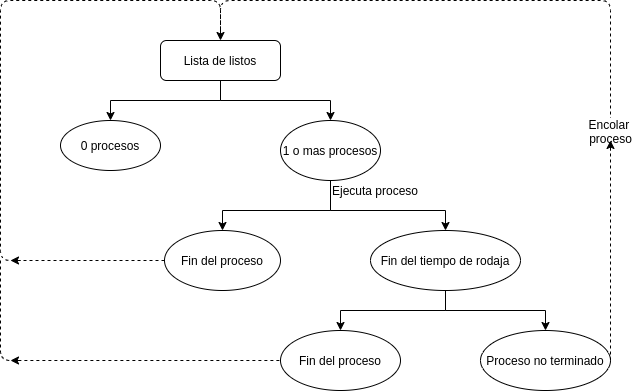
\includegraphics[width=8cm]{arboles/RoundRobin.png}
    \caption{Máquina de estados Round Robin}
\end{figure}

Para poder implementar el planificador Round-Robin en necesario añadir el campo que contabilice los ticks, es decir, las rodajas  de tiempo en el BCP y también es necesario modificar la interrupción de reloj. Por ello:

\subsubsection{Estructuras de datos}
\begin{itemize}
    \item Ticks en el BCP para poder tener en cuenta las rodajas de tiempo.
    \item Lista de listos. En este caso se reutilizara la cola ofrecida en el enunciado de la práctica.
\end{itemize}

\subsubsection{Funciones}
\begin{itemize}
    \item \textbf{mythead\_create (void (*fun\_addr)( ), int priority, int seconds)}
    \begin{itemize}
        \item Crea el proceso que se va a ejecutar
        \item El número de ticks del BCP son el máximo por rodaja
        \begin{itemize}
            \item BCP. ticks = QUANTUM\_TICKS
        \end{itemize}
        \item El estado pasa a estar listo
        \begin{itemize}
            \item BCP.state = INIT
        \end{itemize}
        \item Insertar lista de listos
    \end{itemize}
    
    \item \textbf{TCB *scheduler ( )}
    \begin{itemize}
        \item Si no está vacía la lista de listos:
        \begin{itemize}
            \item Desencola el primer proceso y lo guarda 
            \item Devuelve el proceso
        \end{itemize}
    \end{itemize}
    
    \item \textbf{activator (TCB *next)}
    \begin{itemize}
        \item Si (swap == -1)
        \begin{itemize}
            \item setcontext (nextContext)
        \end{itemize}
        \item Para el resto de los casos
        \begin{itemize}
            \item swapcontext (prev, next)
        \end{itemize}
    \end{itemize}
    
    \item \textbf{timer\_interrupt ( )}
    \begin{itemize}
        \item Running.ticks -= 1
        \item El estado pasa a listo para ejecutar
        \item Ticks = QUANTUM\_TICKS
        \item Encolar en lista de listos
        \item Prev = hilo ejecutado hasta ahora
        \item Llama al planificador (scheduler)
        \item El estado pasa a ejecutando
        \item Activador (hilo ejecutado hasta ahora)

    \end{itemize}
\end{itemize}

\subsection{Round-Robin/ SJF con prioridades}
Una vez analizado el enunciado inicial, la máquina de estados finita resultante para este apartado ha sido la siguiente:

\vspace{0.5cm}
\begin{figure}[h]
    \centering
    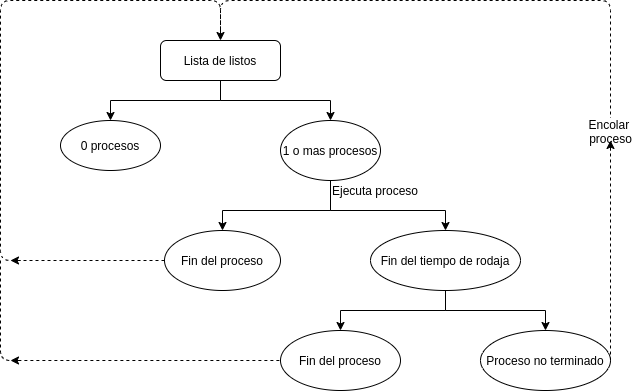
\includegraphics[width=8cm]{arboles/RoundRobin.png}
    \caption{Máquina de estados RRS}
\end{figure}

\subsubsection{Estructuras de datos}
\subsubsection{Funciones}

\subsection{Round-Robin/ SJF con posibles cambios de contexto voluntarios}
Una vez analizado el enunciado inicial, la máquina de estados finita resultante para este apartado ha sido la siguiente:

\newpage
\vspace{0.5cm}
\begin{figure}[!h]
    \centering
    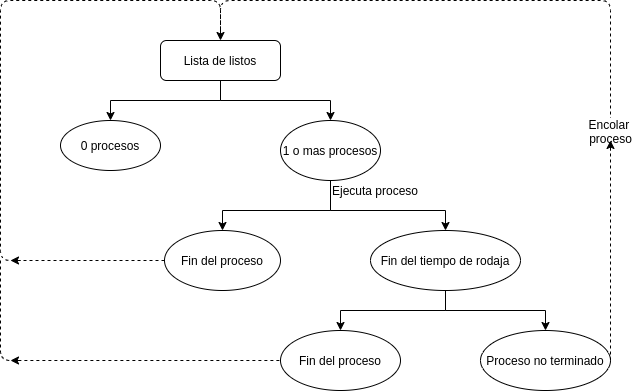
\includegraphics[width=8cm]{arboles/RoundRobin.png}
    \caption{Máquina de estados RRSD}
\end{figure}
\subsubsection{Estructuras de datos}
\subsubsection{Funciones}

\newpage
\section{Batería de pruebas}
Para poder comprobar el código realizado se van a crear una serie de \textbf{árboles para cada planificador}, para poder ir viendo las distintas opciones de ejecución. Cada árbol contendrá todos los posibles casos como nodos terminales. Se han incluido líneas discontinuas para aquellos casos que se puedan repetir, y así poder cerrar el ciclo total de cada ejecución.

Con respecto al código, se ha creado un \textbf{script} de bash denominado \textbf{\textit{pruebas}}, el cual se ejecutará dentro del directorio donde se encuentran todos los ficheros de la práctica. En la clase principal del programa, \textit{main.c}, se han diferenciado todas las posibles pruebas de tal manera que para ejecutar cada una individualmente se hará de la siguiente manera:
       
                                    $$ ./main testX $$

Para una mayor comodidad, todas las pruebas se llaman testX, donde X es el número identificativo de cada prueba.

El script se encargará de, en primer lugar, hacer make y a continuación \textbf{ejecutar todas las pruebas} que han sido implementadas de manera individual, tal y como se ha indicado anteriormente. A lo largo de este punto se irá desarrollando que hace cada prueba, indicando a su vez el nombre otorgado.El \textbf{\textit{test0}} es el test por defecto que se da en el código base de la práctica.

\subsection{Round Robin}
Este caso es el más sencillo a la hora de crear el árbol, ya que no se tiene en cuenta la prioridad del proceso, sino que se encolan todos de igual manera y se van ejecutando en función a una rodaja de tiempo predeterminada. Por ello, el árbol sera el siguiente:

\vspace{0.5cm}
\begin{figure}[h]
    \centering
    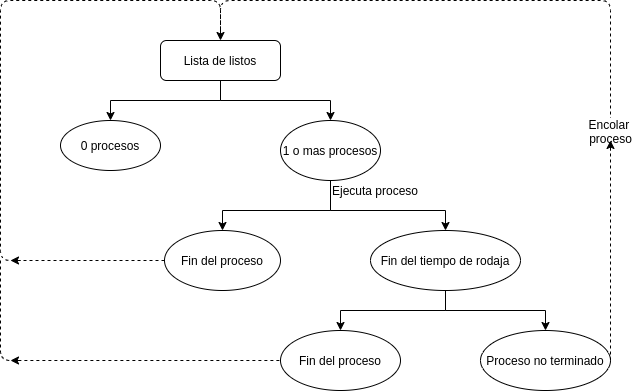
\includegraphics[width=10cm]{arboles/RoundRobin.png}
    \caption{Árbol de pruebas Round Robin.}
\end{figure}

Como se puede ver, hay 2 opciones: que la \textbf{lista de listos está vacía} o tenga algún proceso. En caso de estar vacía, \textbf{termina la ejecución}. Por otro lado, en caso de tener 1 o más procesos se ejecuta cada proceso el tiempo indicado en QUANTUM\_TICKS. En caso de terminar el proceso antes de finalizar dicha rodaja de tiempo, finaliza la ejecución y analizará nuevamente la lista de listos (se implementa como \textbf{\textit{test1}}).  

En caso de \textbf{finalizar} el tiempo marcado por cada \textbf{rodaja} pueden darse dos casos: que se haya terminado de ejecutar el hilo, a la par que termina el tiempo (caso implementado como \textbf{\textit{test2}}), o que aún no haya terminado su ejecución (caso implementado como \textbf{\textit{test3}}). En el primer caso, se terminará la ejecución de dicho hilo y se procederá a \textbf{analizar la lista de listos nuevamente}. En el segundo caso, el proceso volverá a poner el número de rodaja en su totalidad y será \textbf{encolado} en la lista de listos, procediendo a analizar, nuevamente, la lista de listos.

Si llega un proceso durante la ejecución de otro proceso se encola con su rodaja correspondiente en la lista de listos a continuación (caso implementado como \textbf{\textit{test4}}).

\subsection{Round-Robin/ SJF con prioridades}
El árbol creado para este caso ha sido el siguiente:
\vspace{0.5cm}
\begin{figure}[h]
    \centering
    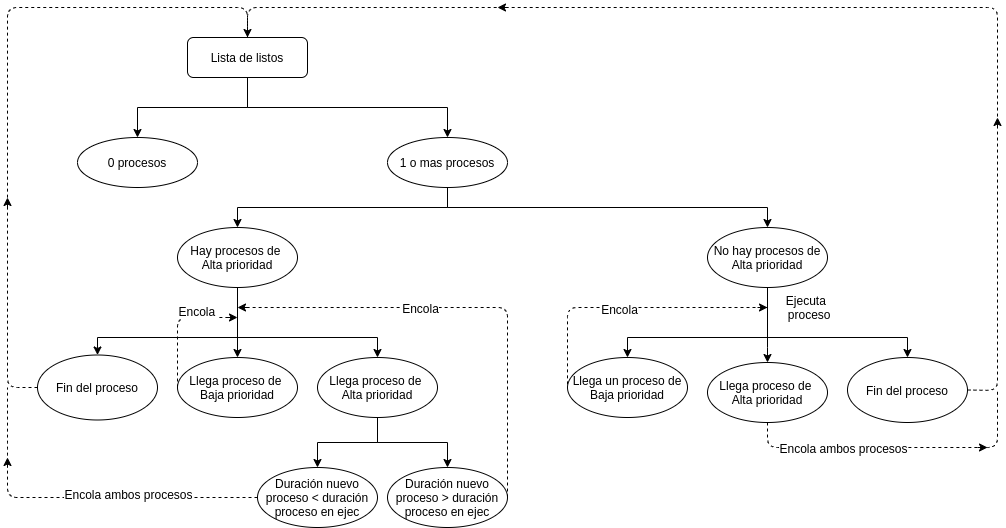
\includegraphics[width=14cm]{arboles/RRS.png}
    \caption{Árbol de pruebas RRS}
\end{figure}

En primer lugar, nuevamente se analiza la lista de listos para ver qué proceso va a ejecutarse. En caso de no haber procesos pendientes finaliza la ejecución. En el caso de existir algún proceso en la lista de listos, en \textbf{primer lugar} se ejecutarán aquellos procesos de \textbf{alta prioridad}. Para comprobar que esto se cumple, se ha creado una prueba donde hay varios procesos en la cola, tanto de alta como de baja prioridad (caso implementado como \textbf{\textit{test5}}). 

Si mientras se ejecuta un proceso de alta prioridad entra un proceso de \textbf{baja prioridad}, se mete este último en la lista de listos y \textbf{continúa} ejecutándose el primer proceso . En caso de entrar otro proceso de \textbf{alta prioridad}, sería necesario \textbf{comparar la duración} de este. Si la duración del nuevo proceso es \textbf{mayor} o igual que la del proceso en ejecución, se encola el último proceso y se \textbf{continúa} con la ejecución del proceso inicial (caso implementado como \textbf{\textit{test6}}). Si por el contrario la duración es menor, se encolan ambos en la lista de listos, donde se ordenarán por el menor trabajo primero (caso implementado como \textbf{\textit{test7}}). Si termina la ejecución del proceso se vuelve a analizar la lista de listos.

Por otro lado, si al analizar la lista de listos no hay procesos de alta prioridad pero sí de \textbf{baja prioridad}, pasan a ejecutarse en orden según la política \textbf{Round Robin}. Mientras se ejecuta el proceso puede darse el caso en que entre un proceso de \textbf{alta prioridad} o de baja prioridad. En el primer caso, dejará de ejecutarse el proceso actual, reiniciando la rodaja y encolándose en la lista de listos de baja prioridad. En ese momento \textbf{se comenzaría a ejecutar} el proceso de alta prioridad, puesto que al analizar la lista de listos es el que tiene prioridad (caso implementado como \textbf{\textit{test8}}).

En caso de encontrarse ejecutando un proceso de \textbf{baja prioridad} y entra otro de la misma prioridad, este \textbf{se encolaría} en la lista de listos de los procesos de baja prioridad para ser ejecutado en su momento (caso implementado como \textbf{\textit{test9}}). Si el proceso que se está ejecutando consume el tiempo total de la rodaja, se encola reiniciando nuevamente dicho valor y se vuelve a analizar la lista de listos. También analiza la lista de listos cuando el proceso haya terminado.


\subsection{Round-Robin/ SJF con posibles cambios de contexto voluntarios}
Para el siguiente árbol se ha partido del árbol adjunto en el apartado anterior:

\vspace{0.5cm}
\begin{figure}[h]
    \centering
    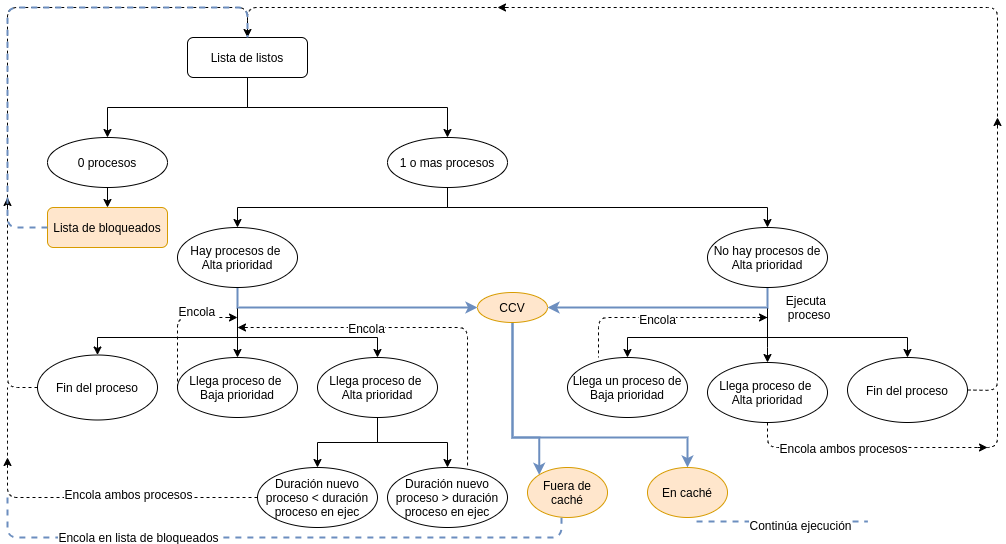
\includegraphics[width=15cm]{arboles/RRSD.png}
    \caption{Árbol de pruebas RRSD}
\end{figure}

Las diferencias se encuentran marcadas de otro color: rojo para los nodos y azul para los diversos enlaces. Como se puede apreciar, se han añadido los casos para los \textbf{cambios de contexto voluntarios} (indicados en la imagen como CCV). Puesto que el código también se reutiliza, aquellas pruebas que resulten repetitivas no se han ejecutado.

Durante la ejecución de un proceso este puede requerir un cambio voluntario. Si la información que requiere el proceso se encuentra \textbf{en caché}, el proceso tomará dichos datos y \textbf{continuará} su ejecución sin realizar ninguna acción más (caso implementado como \textbf{\textit{test10}} y \textbf{\textit{test11}}, dependiendo si parte de un proceso de prioridad alta o de prioridad baja). Si por el contrario la información requerida \textbf{no} se encontrase \textbf{en memoria caché}, el proceso se añadiría a la \textbf{lista de bloqueados} y pasaría a analizar la lista de listos para ejecutar el siguiente proceso (caso implementado como \textbf{\textit{test12}}).

En caso de no darse mas procesos a ejecutar en la lista de listos, si la lista de bloqueados no se encuentra vacía se pondrá en ejecución el \textbf{thread \textit{idle}}. Este thread ejecutará un bucle infinito, de tal forma que el planificador consulte cada tick de reloj si existe algún thread listo para ejecutar, tal y como se indica en el enunciado de la práctica (caso implementado como \textbf{\textit{test13}}). 

Con respecto a la imagen, aunque se haya indicado que da igual si parte de la ejecución de procesos de alta prioridad o de los procesos de baja prioridad a la hora de realizar el cambio de contexto voluntario, esto no es cierto. En caso de contener los datos en la caché, al continuar la ejecución se continuará dependiendo de su prioridad en una rama del árbol o en otra. En la imagen no se ha dividido para poder ahorrar espacio y que así se pudiera ver mejor.

\vspace{1cm}
\section{Resultados batería de pruebas}

\newpage
\section{Conclusiones}

\end{document}
